\documentclass[12pt,letterpaper,oneside]{report}
\usepackage[T1]{fontenc}
\usepackage[utf8]{inputenc}
\usepackage[spanish]{babel}
\usepackage{amsmath,amsfonts,amsthm}
\usepackage{titlesec}
\usepackage{graphicx}
\usepackage{multicol}
\usepackage{enumitem}
\usepackage{xspace}
\usepackage[papername={letterpaper},top=3cm,bottom=3cm,left=3cm,right=3cm]{geometry}

\setlength{\parindent}{0pt}
\titleformat{\chapter}{\Huge\bfseries}{\thechapter}{1em}{}

\newcommand{\thetitle}{Resistencia celular y tiempo de respuesta imunológica en un modelo para la infección del VIH}

\newcommand{\theteacher}{Juárez Martínez Genaro}

\newcommand{\theassignment}{Computer Selected Topics}

\newcommand{\thedate}{Julio 8, 2015}

\begin{document}
	\begin{titlepage}

\centering
\vspace*{3cm}
\includegraphics[width=3.5cm]{/home/iann/Documentos/Escom/ipn_logo2.jpg}\\[0.5cm]
\Large Instituto Politécnico Nacional\xspace\\
\Large Escuela Superior de Cómputo\xspace\\[0.3cm]
\vspace{1cm}
\Large \theassignment
\par

\huge\thetitle
\vfill

\large\flushright
\textbf{Elaborado por:}\\
Hernández Sánchez Ian Yevgeni\\[0.5cm]

\textbf{Profesor:}\\
\theteacher\\[1cm]
\vfill

\normalsize
\thedate

\end{titlepage}
	\tableofcontents

	\chapter{Introducción}
	El curso de infección del VIH se caracteriza por la existencia de dos periodos principales:
	\begin{itemize}
		\item Periodo de infección
		\item Periodo de latencia
	\end{itemize}

	Se considera que el paciente ha adquirido el SIDA cuando el conteo de células-T baja hasta encontrarse entre el 20\% y el 30\%.\\

	Este modelo utiliza formalismos de autómatas celulares para describir la propagación de la infección en tejido linfoide y reproduce la dinámica de tres estados observada en pacientes infectados. También, podemos observar que se forman estructuras de células infectadas propagadas por el tejido, atrapando células sanas y destruyendo el tejido.\\

	\section{Modelo del autómata celular} % (fold)
	\label{sec:modelo_del_aut_mata_celular}
	Se representa la estructura de los nodos linfáticos mediante un espacio cuadrado de $L\ \chi\ L$, cada uno de los elementos del espacio representa una célula, la cual tiene 4 estados posibles:
	\begin{enumerate}
		\item \textbf{Célula sana:} Representa a las células $CD4^{+}$ y macrófagas.
		\item \textbf{Célula infectada-A:} Son las que han sido infectadas recientemente y no han sido reconocidas por el sistema inmunológico.
		\item \textbf{Célula infectada-B:} Son células infectadas-A, las cuales después de un tiempo ha perdido la capacidad para propagar la infección.
		\item \textbf{Célula muerta:} Son células que han muerto a causa de la infección.\\
	\end{enumerate}

	La configuración inicial se compone en su mayoría de células sanas, con una pequeña fracción $P_{VIH}=0.05$ de células infectadas-A, distribuidas de manera aleatoria en el espacio.

	\newpage
	Las siguientes reglas se aplican en cada periodo de tiempo transcurrido:
	\begin{enumerate}
		\item Una célula sana se convierte en infectada-A si tiene al menos $R_a$ células vecinas infectadas-A o $R_b$ células vecinas infectadas-B. De lo contrario permanece sana.

		Esta regla toma en cuenta la propagación de la infección a causa del contacto entre células. En el modelo original $R_a = 1$ y $R_b = 4$.\\

		\item Una célula infectada-A propaga la infección durante $\tau$-periodos de tiempo, luego se convierte en infectada-B.

		El tiempo de respuesta $\tau$ es el tiempo que necesita el sistema inmunológico para desarrollar un determinado antígeno y puede variar de 1 a 8 semanas. En el modelo original $\tau = 4$ para todas las células infectadas-A.\\

		\item Una célula infectada-B muere después de un periodo de tiempo.\\
		\item Una célula muerta tiene una probabilidad $P_{repl}$ de ser reemplazada por una célula nueva, dicha célula nueva tiene $P_{infec}$ probabilidades de ser infectada-A y $1 - P_{infec}$ probabilidades de ser sana. En el modelo original $P_{repl} = 0.99$ y $P_{infec} = 10^{-5}$.
	\end{enumerate}
	% section modelo_del_aut_mata_celular (end)

	\section{Variables del modelo} % (fold)
	\label{sec:variables_del_modelo}
	El objetivo de este proyecto es observar los cambios ocurridos en el comportamiento del sistema cuando se modifican las variables del modelo para simular escenarios diferentes al planteado. Como se menciona, las variables que se buscan modificar son la ``Resistencia celular'' y el ``Tiempo de respuesta inmunológica'', para esto se deben modificar los parámetros cuyos valores están involucrados en estos procesos.\\

	Para variar la Resistencia celular, se deben modificar los valores de $R_a$ y $R_b$, al hacer más altos estos parámetros estamos simulando una mayor resistencia celular en el paciente y viceversa.\\

	Para el caso del Tiempo de respuesta inmunológica, se debe modificar el valor de $\tau$, mientras más alto sea su valor, mayor es el tiempo que le toma al sistema inmunológico detectar a las células infectadas.
	% section variables_del_modelo (end)


    \chapter{Desarrollo}
    \section{Tecnologías de desarrollo} % (fold)
	\label{sec:tecnolog_as_de_desarrollo}
	\subsubsection{Vala}
	Es un lenguaje de programación orientado a objetos que utiliza el sistema \emph{GObject}. Su compilador, \emph{valac}, genera código en C a partir del escrito en Vala para después compilar el código generado usando un compilador como \emph{gcc}. Su sintaxis es similar a la de C\#.\\
	
	\subsubsection{GTK+}
	Es un conjunto de bibliotecas multiplataforma para desarrollar interfaces gráficas de usuario (GUI), principalmente para los entornos gráficos GNOME, XFCE y ROX aunque también se puede usar en el escritorio de Windows, Mac OS y otros. Es una de las más utilizadas en entornos gráficos de escritorio para ambientes Unix.\\
	% section tecnolog_as_de_desarrollo (end)

	\section{Interfaz gráfica de usuario} % (fold)
	\label{sec:interfaz_gr_fica_de_usuario}
    La aplicación fue desarrollada en el lenguaje de programación Vala, ejecuta una interfaz gráfica hecha en GTK+ en la cual están presentes tanto el espacio que muestra las iteraciones del autómata como la sección que contiene los controles para ajustar los parámetros de ejecución. Dentro de los controles tenemos widgets para cambiar el tamaño del espacio, el porcentaje de infección inicial, los parámetros $R_a$, $R_b$ y $\tau$, así como un espacio en el que se muestra información acerca del estado actual del autómata, tal como:
    \begin{itemize}
    	\item Porcentaje de células vivas.
    	\item Porcentaje de células infectadas.
    	\item Porcentaje de células muertas.
    	\item El número de iteraciones que han transcurrido.
    \end{itemize}
	
	De igual manera incluye botones para generar la configuración inicial del espacio, limpiar el espacio y para iniciar/pausar la simulación.

	\begin{figure}[h!]
		\centering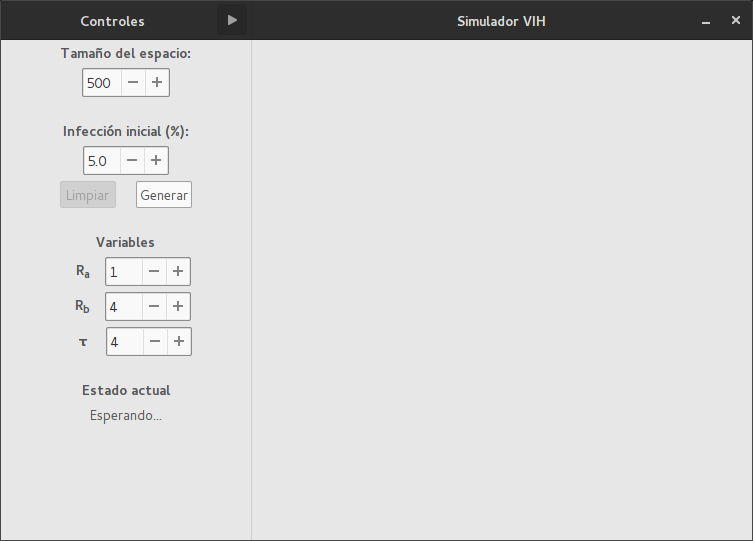
\includegraphics[height=8cm]{img/main.png}
		\caption{Ventana principal de la aplicación.}
	\end{figure}~\\

	También, se puede desplegar un cuadro de diálogo sobre la ventana principal donde se muestra la gráfica generada a partir de los porcentajes de células vivas, infectadas y muertas hasta el momento.
	\begin{figure}[h!]
		\centering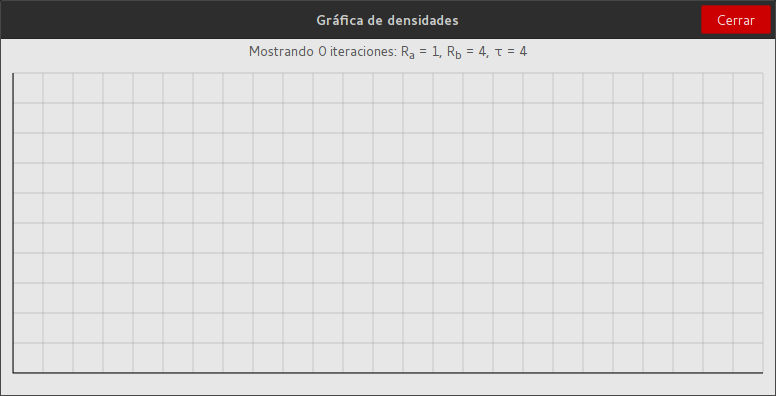
\includegraphics[width=12cm]{img/grafica.png}
		\caption{Cuadro de diálogo para la gráfica de densidades.}
	\end{figure}
	% section interfaz_gr_fica_de_usuario (end)

	\chapter{Pruebas del modelo original}
	Para todas las simulaciones y pruebas a partir de esta sección se utilizará un espacio con $L = 500$, se tomarán como ejemplo 4 capturas durante la ejecución de la simulación en tiempos similares para compararlas. Se realizarán simulaciones de 250 iteraciones cada una.\\

	Dentro del espacio del autómata se tienen 4 colores para representar cada estado posible de las células, el azul representa las células sanas, el amarillo a las células infectadas-A, el verde a las células infectadas-B y el rojo a las células muertas.\\

	En las gráficas de densidades, la línea azul representa a las células sanas, la línea verde a las infectadas tanto de tipo A como de tipo B y la línea roja a las células muertas.

	\section{Parámetros originales} % (fold)
	\label{sec:par_metros_originales}
	Para las pruebas de esta sección se dejarán los parámetros de ejecución en sus valores por defecto ($R_a = 1,\ R_b = 4,\ \tau = 4$).

	\subsection{Simulación en ejecución} % (fold)
	\label{sub:simulaci_n_en_ejecuci_n}
	\begin{center}
		\begin{tabular}{c c}
		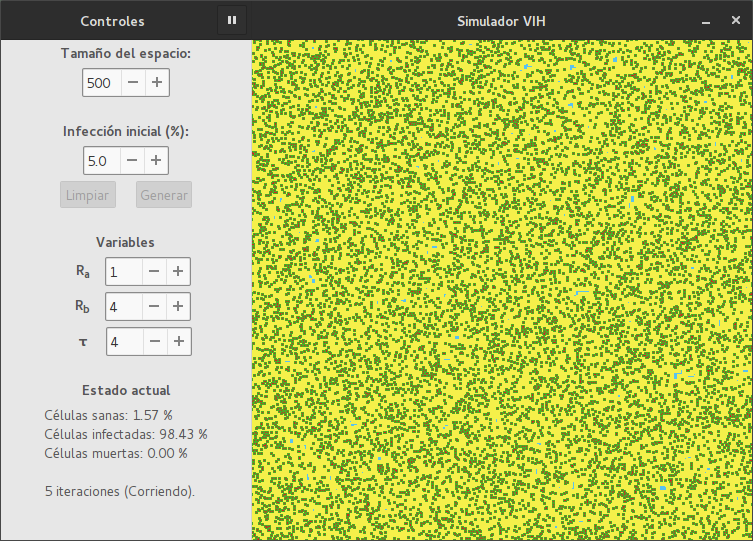
\includegraphics[width=8cm]{img/original/prueba/1.png} & 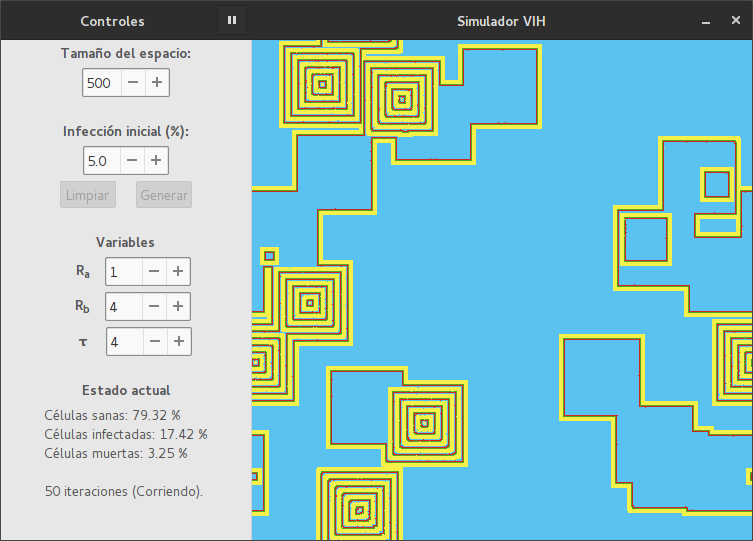
\includegraphics[width=8cm]{img/original/prueba/2.png} \\
		\end{tabular}
	\end{center}

	\begin{center}
		\begin{tabular}{c c}
		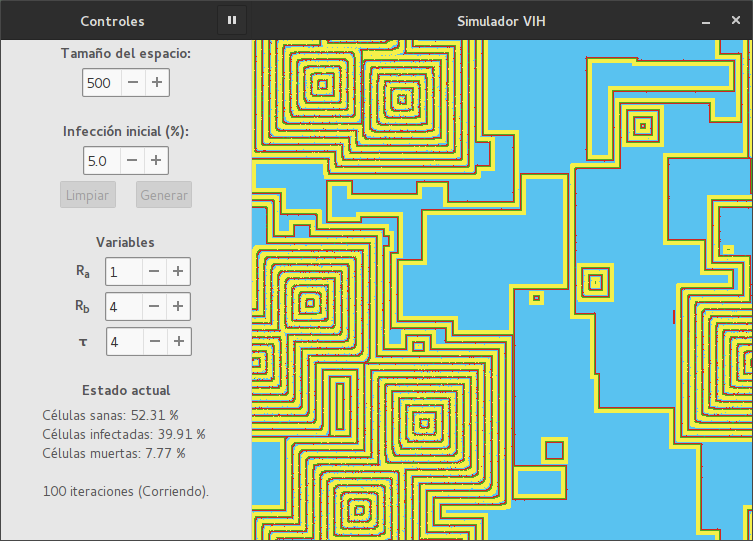
\includegraphics[width=8cm]{img/original/prueba/3.png} & 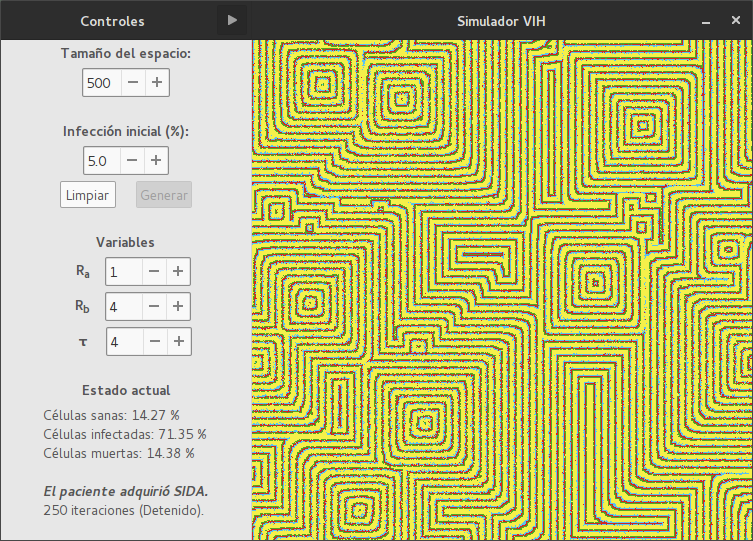
\includegraphics[width=8cm]{img/original/prueba/4.png} \\
		\end{tabular}
	\end{center}

	\subsubsection{Gráfica de densidades}
	\begin{center}
		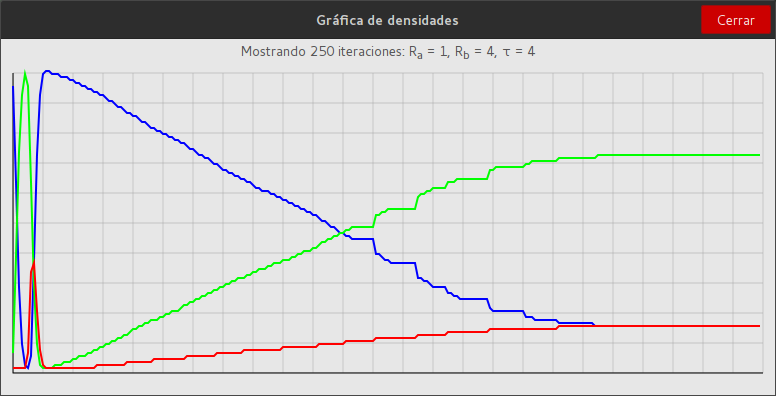
\includegraphics[width=14cm]{img/original/prueba/g.png}
	\end{center}
	% subsection simulaci_n_en_ejecuci_n (end)
	% section par_metros_originales (end)

	\section{Casos extremos} % (fold)
	Para este caso, como casos extremos se variarán los porcentajes de infección inicial tomando un $1.0\%$ como el mínimo y un $8.0\%$ como máximo.
	\label{sec:casos_extremos_1}
	\subsection{Con infección inicial mínima} % (fold)
	\label{sub:con_infecci_n_inicial_m_nima}
	\begin{center}
		\begin{tabular}{c c}
		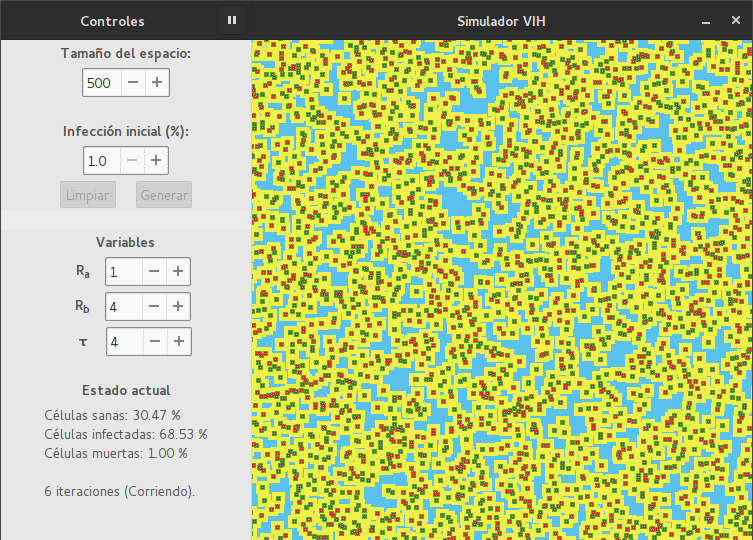
\includegraphics[width=8cm]{img/original/min/1.png} & 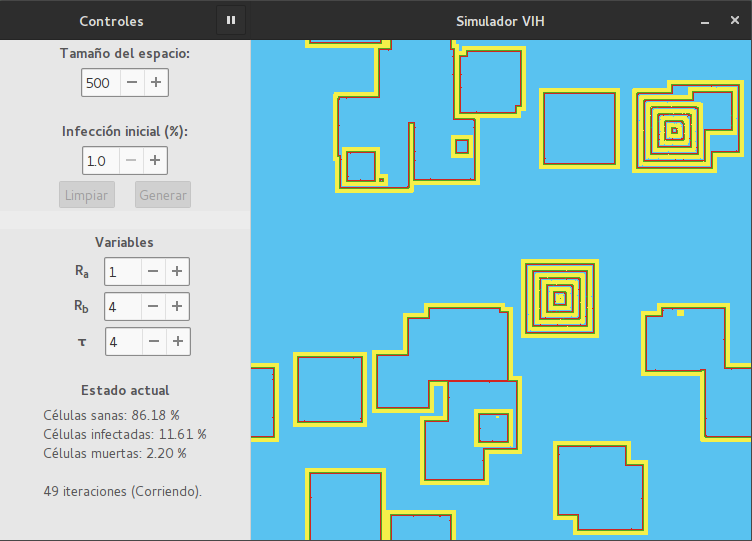
\includegraphics[width=8cm]{img/original/min/2.png} \\
		\end{tabular}
	\end{center}

	\begin{center}
		\begin{tabular}{c c}
		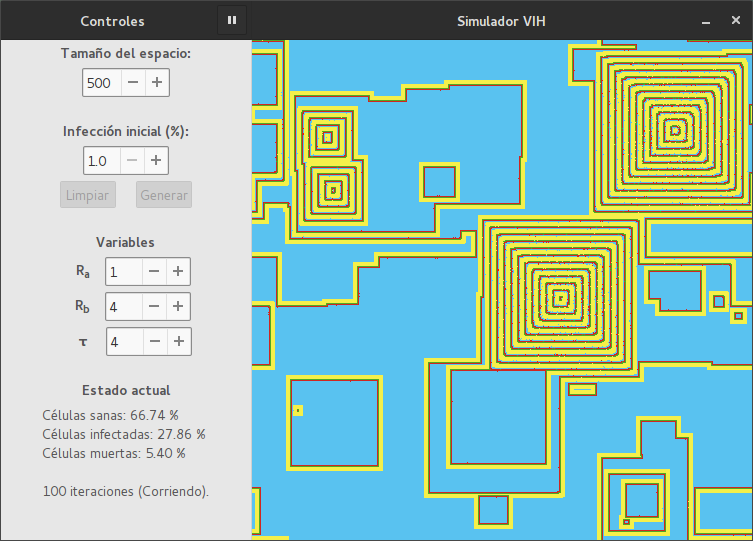
\includegraphics[width=8cm]{img/original/min/3.png} & 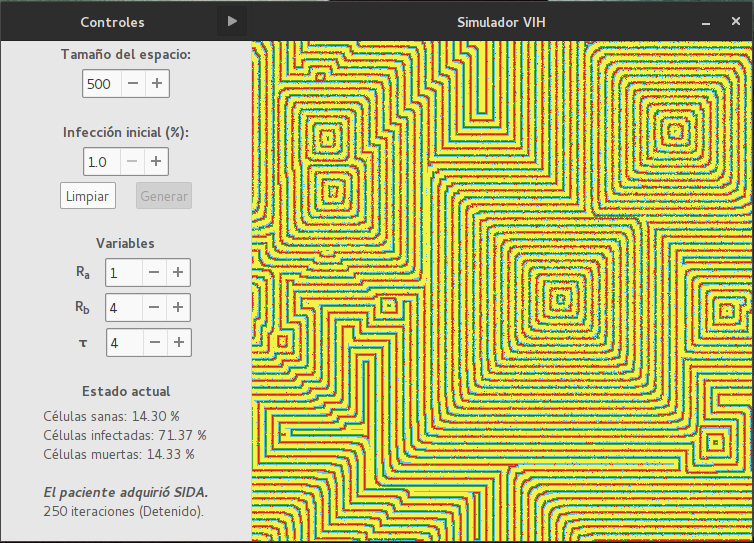
\includegraphics[width=8cm]{img/original/min/4.png} \\
		\end{tabular}
	\end{center}

	\subsubsection{Gráfica de densidades}
	\begin{center}
		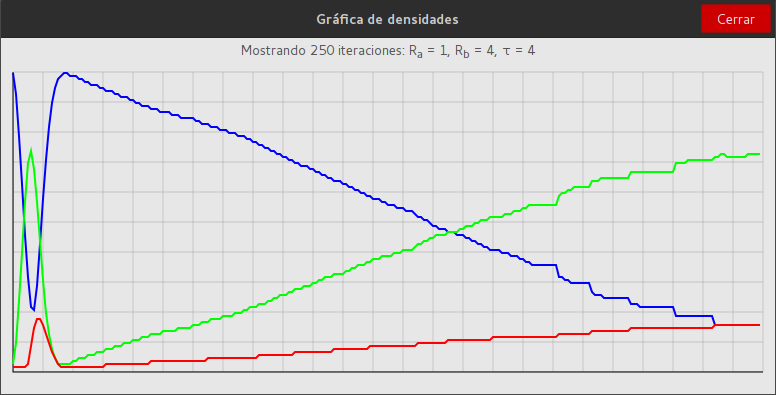
\includegraphics[width=14cm]{img/original/min/g.png}
	\end{center}
	% subsection con_infecci_n_inicial_m_nima (end)

	\subsection{Con infección inicial máxima} % (fold)
	\label{sub:con_infecci_n_inicial_m_xima}
	\begin{center}
		\begin{tabular}{c c}
		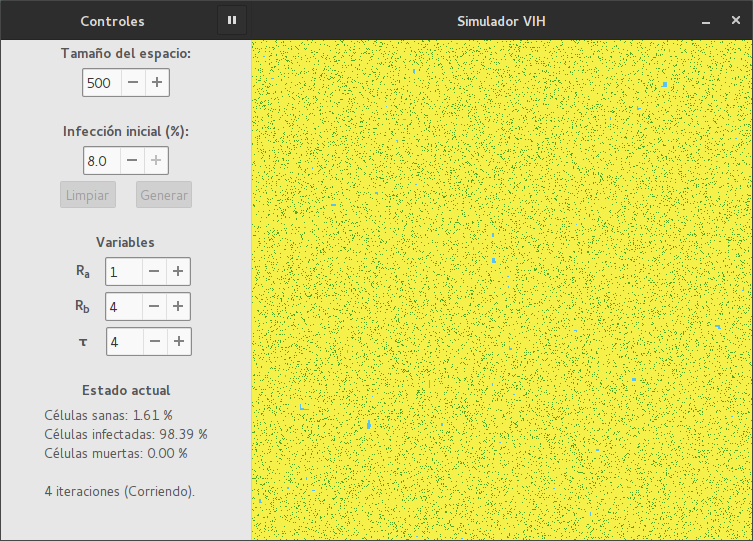
\includegraphics[width=8cm]{img/original/max/1.png} & 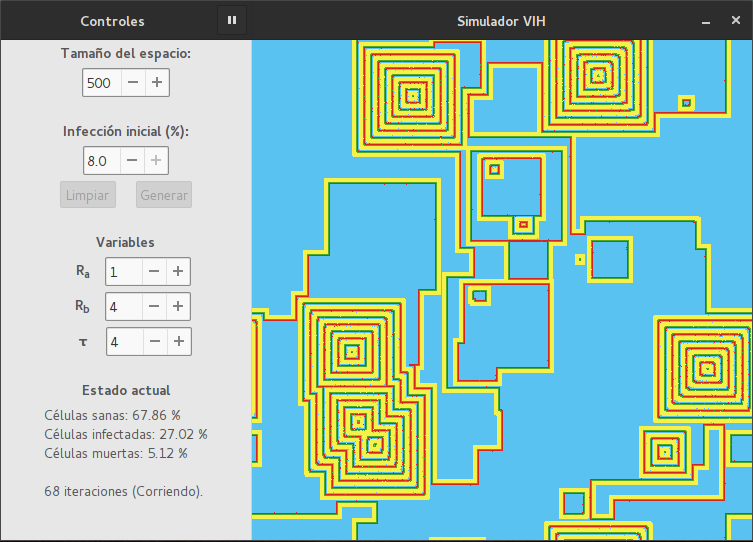
\includegraphics[width=8cm]{img/original/max/2.png} \\
		\end{tabular}
	\end{center}

	\begin{center}
		\begin{tabular}{c c}
		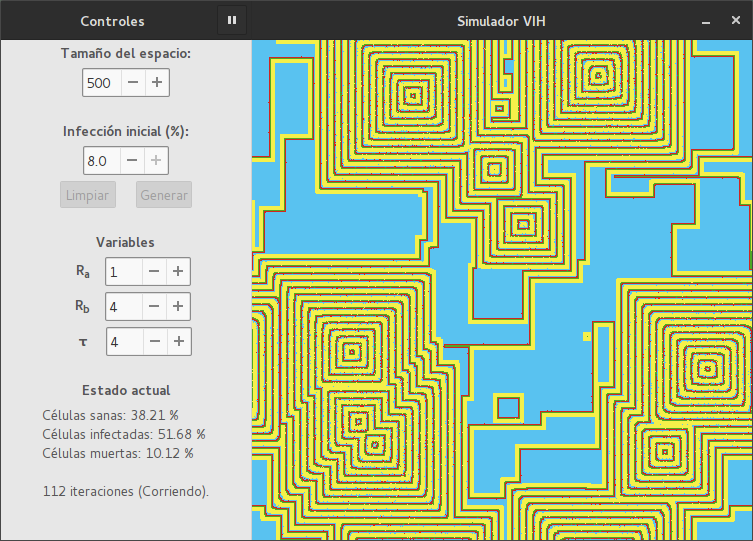
\includegraphics[width=8cm]{img/original/max/3.png} & 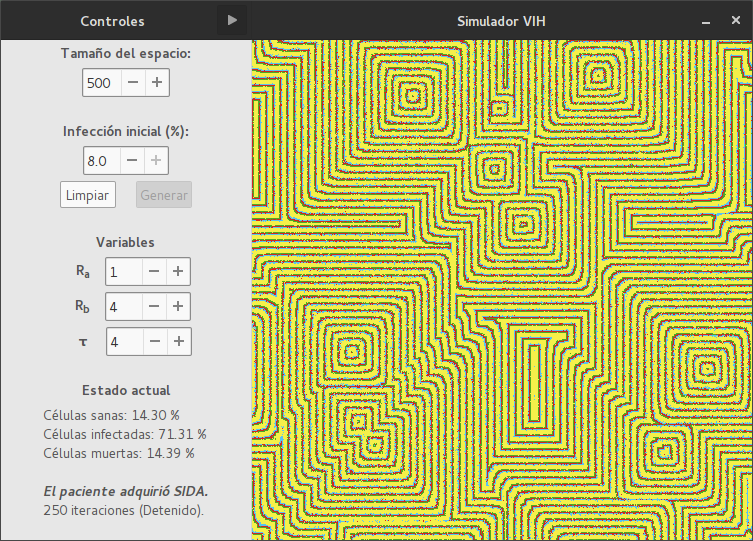
\includegraphics[width=8cm]{img/original/max/4.png} \\
		\end{tabular}
	\end{center}

	\subsubsection{Gráfica de densidades}
	\begin{center}
		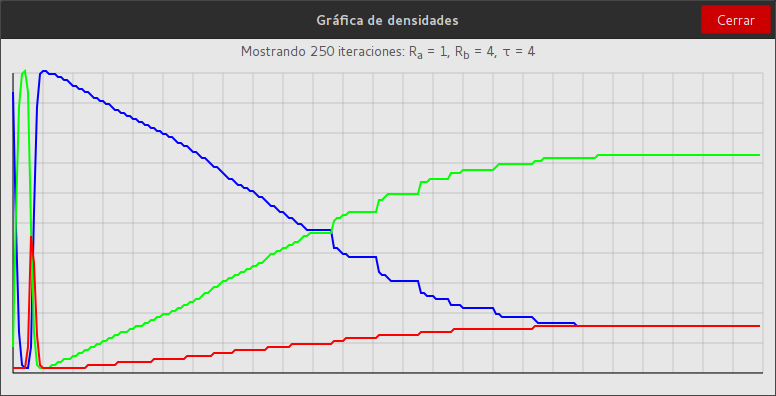
\includegraphics[width=14cm]{img/original/max/g.png}
	\end{center}
	% subsection con_infecci_n_inicial_m_xima (end)
	% section casos_extremos (end)


	\chapter{Variando la resistencia celular}
	\section{Menor resistencia celular} % (fold)
	\label{sec:menor_resistencia_celular}
	\begin{center}
		\begin{tabular}{c c}
		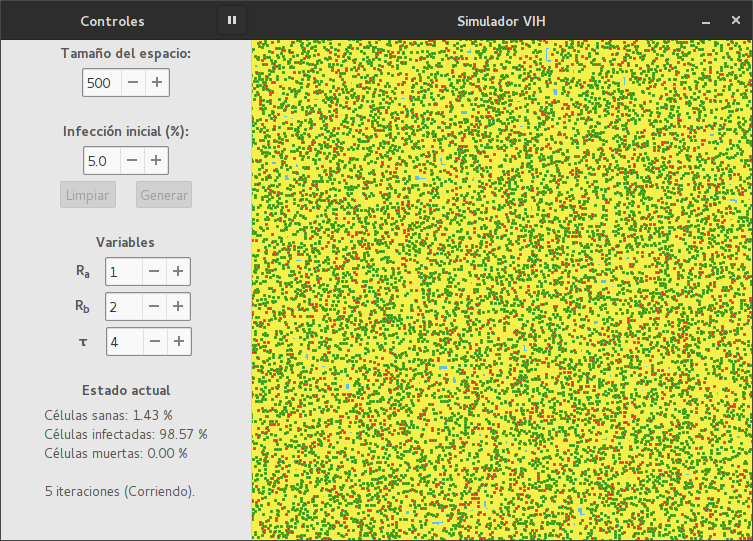
\includegraphics[width=8cm]{img/resistencia/prueba/baja/1.png} & 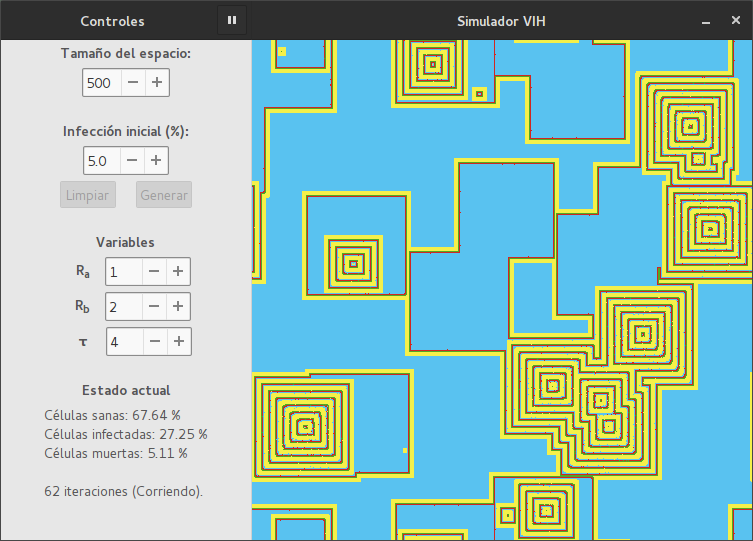
\includegraphics[width=8cm]{img/resistencia/prueba/baja/2.png} \\[1cm]
		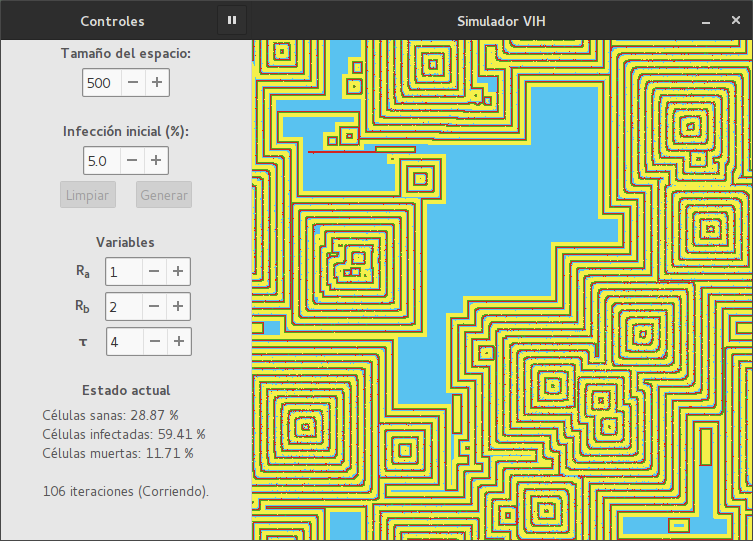
\includegraphics[width=8cm]{img/resistencia/prueba/baja/3.png} & 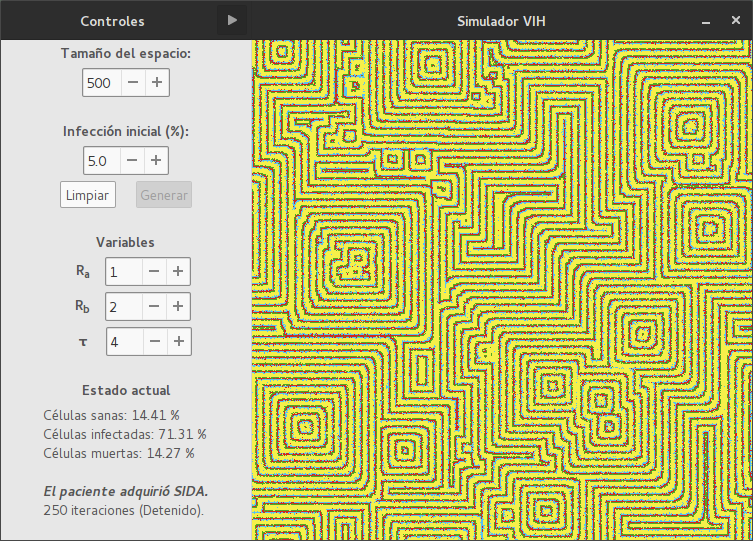
\includegraphics[width=8cm]{img/resistencia/prueba/baja/4.png} \\
		\end{tabular}
	\end{center}

	\subsubsection{Gráfica de densidades}
	\begin{center}
		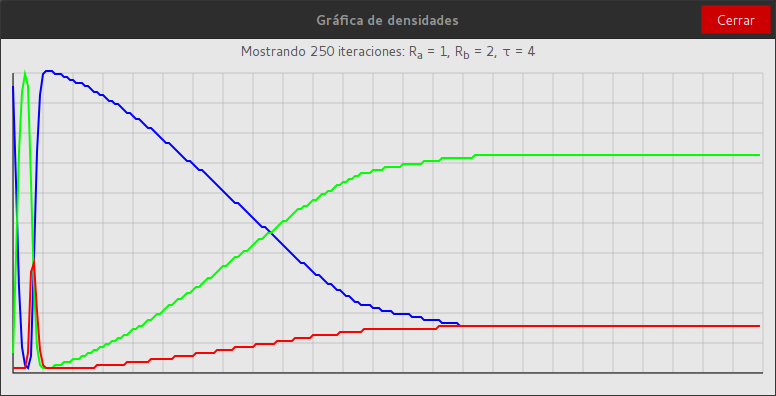
\includegraphics[width=14cm]{img/resistencia/prueba/baja/g.png}\\[3cm]
	\end{center}
	% section menor_resistencia_celular (end)

	\section{Mayor resistencia celular} % (fold)
	\label{sec:mayor_resistencia_celular}
	\begin{center}
		\begin{tabular}{c c}
		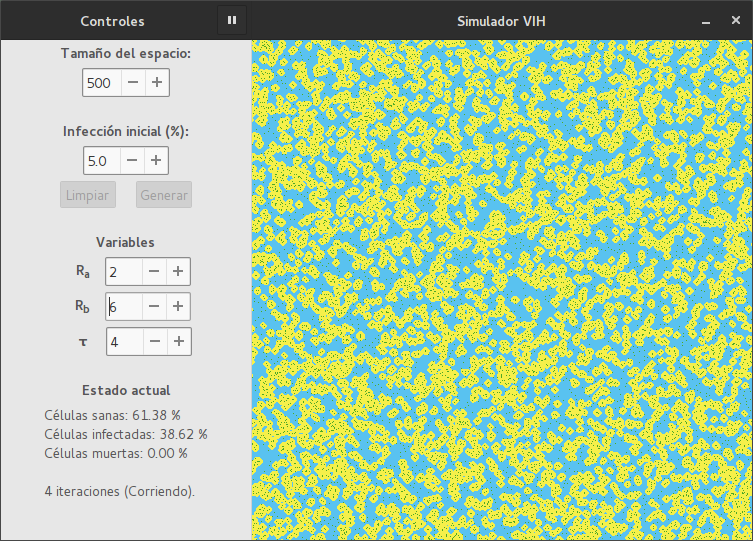
\includegraphics[width=8cm]{img/resistencia/prueba/alta/1.png} & 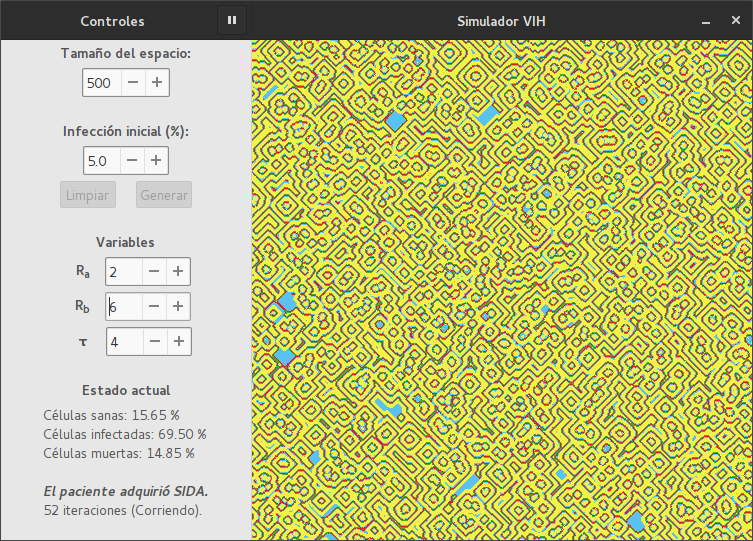
\includegraphics[width=8cm]{img/resistencia/prueba/alta/2.png} \\
		\end{tabular}
	\end{center}
	
	\begin{center}
		\begin{tabular}{c c}
		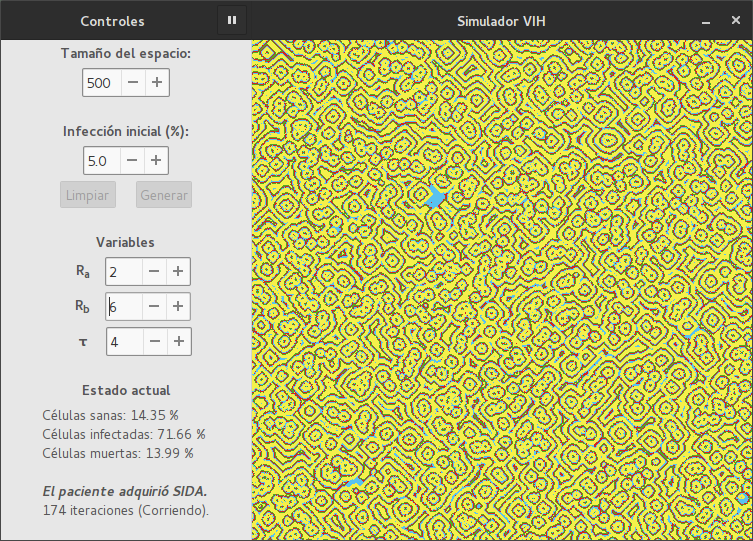
\includegraphics[width=8cm]{img/resistencia/prueba/alta/3.png} & 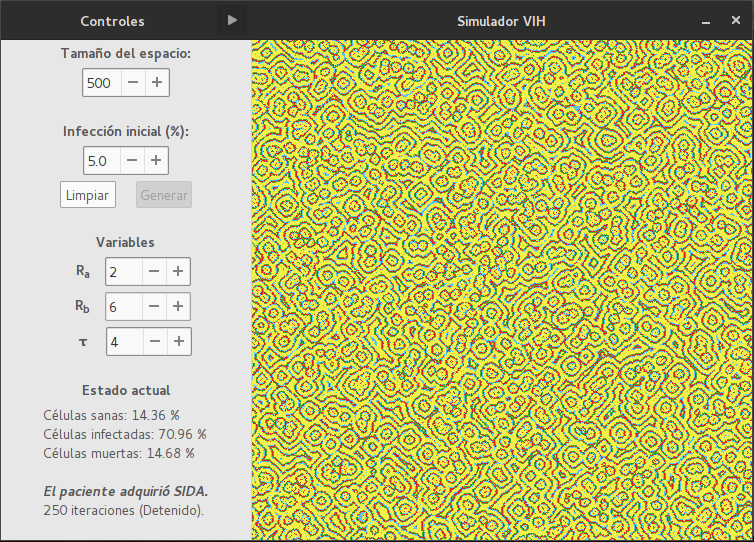
\includegraphics[width=8cm]{img/resistencia/prueba/alta/4.png} \\[1cm]
		\end{tabular}
	\end{center}

	\subsubsection{Gráfica de densidades}
	\begin{center}
		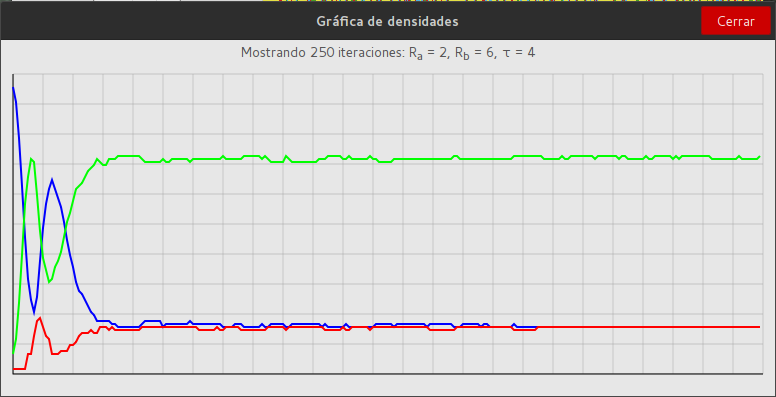
\includegraphics[width=14cm]{img/resistencia/prueba/alta/g.png}
	\end{center}
	% section mayor_resistencia_celular (end)

	\section{Casos extremos} % (fold)
	\label{sec:casos_extremos_2}
	\subsection{Resistencia celular mínima} % (fold)
	\label{sub:resistencia_celular_m_nima}
	\begin{center}
		\begin{tabular}{c c}
		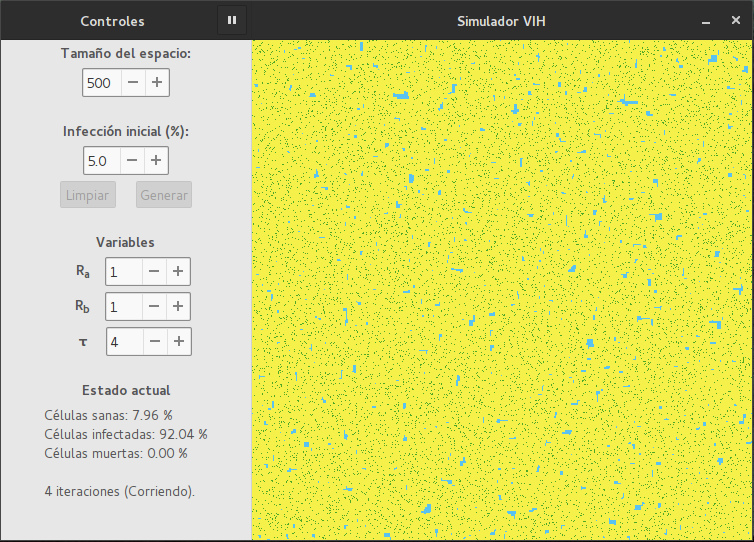
\includegraphics[width=8cm]{img/resistencia/min/1.png} & 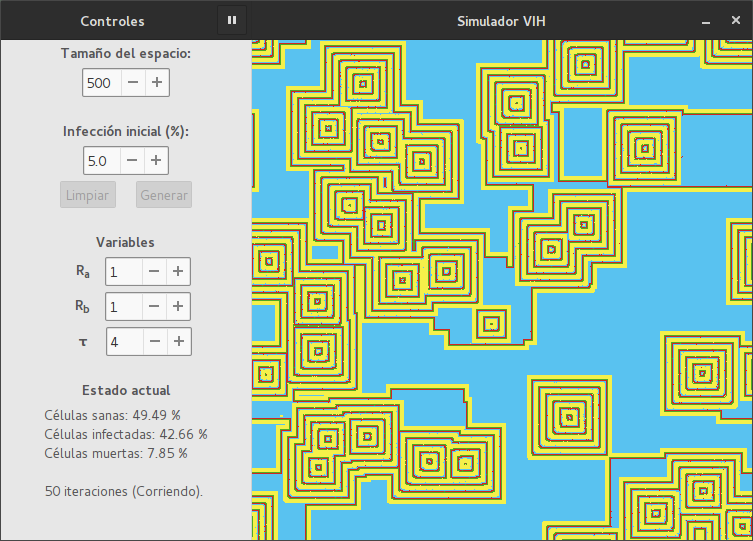
\includegraphics[width=8cm]{img/resistencia/min/2.png} \\
		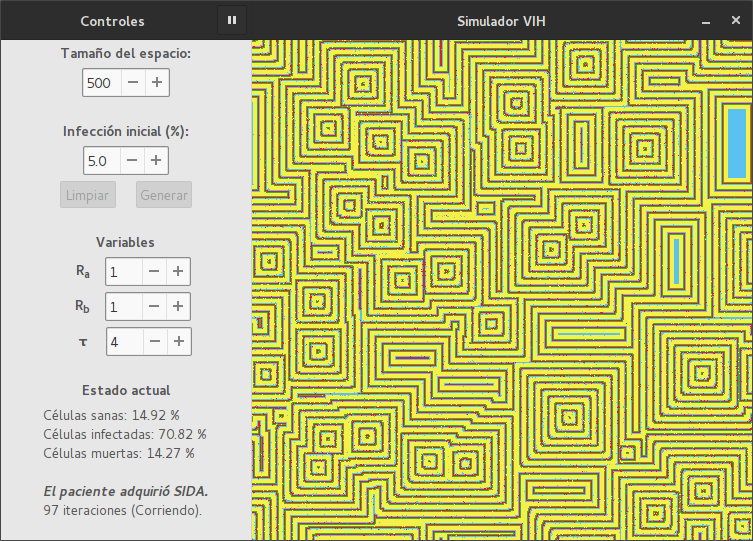
\includegraphics[width=8cm]{img/resistencia/min/3.png} & 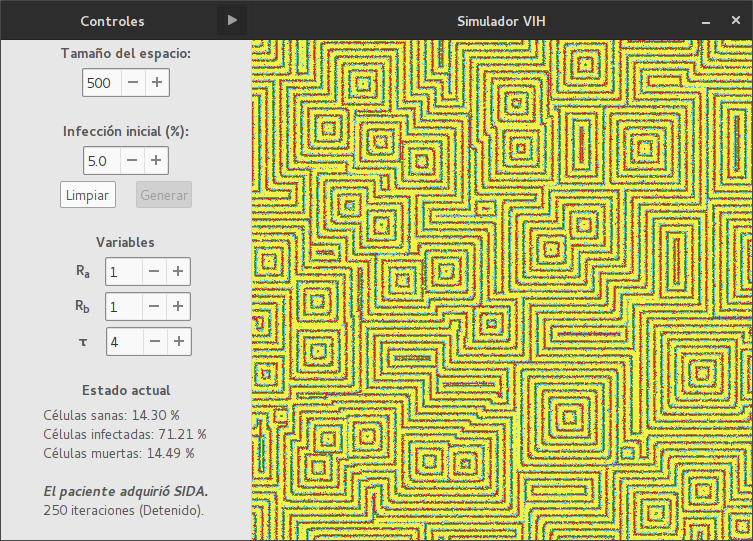
\includegraphics[width=8cm]{img/resistencia/min/4.png} \\
		\end{tabular}
	\end{center}

	\subsubsection{Gráfica de densidades}
	\begin{center}
		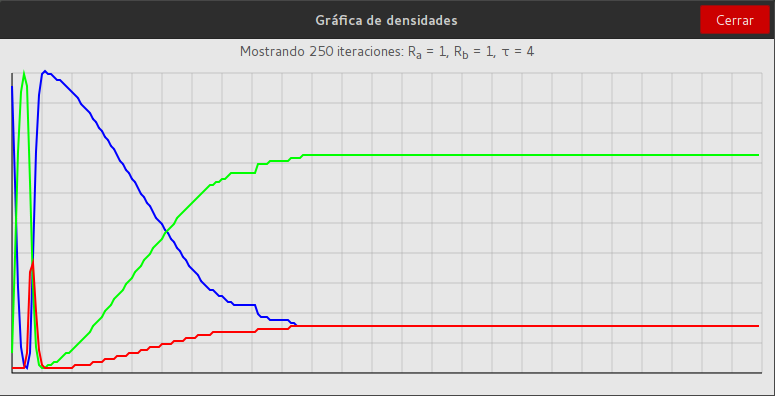
\includegraphics[width=12cm]{img/resistencia/min/g.png}
	\end{center}
	% subsection resistencia_celular_m_nima (end)

	\subsection{Resistencia celular máxima} % (fold)
	\label{sub:resistencia_celular_m_xima}
	\begin{center}
		\begin{tabular}{c c}
		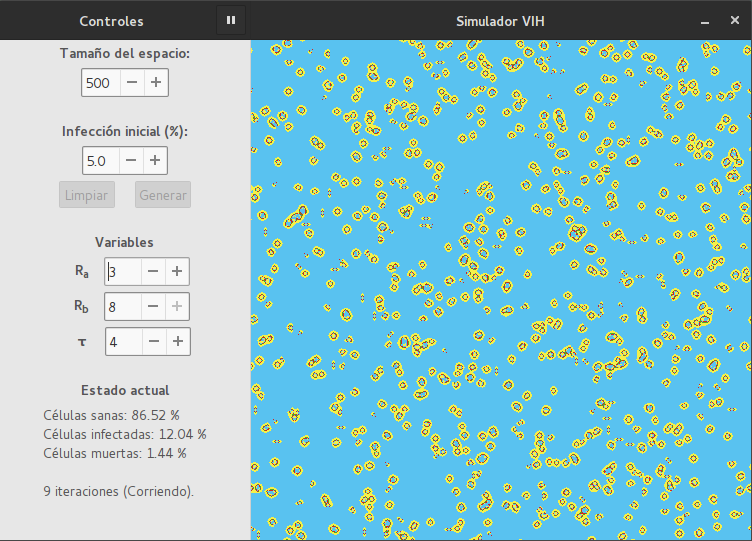
\includegraphics[width=8cm]{img/resistencia/max/1.png} & 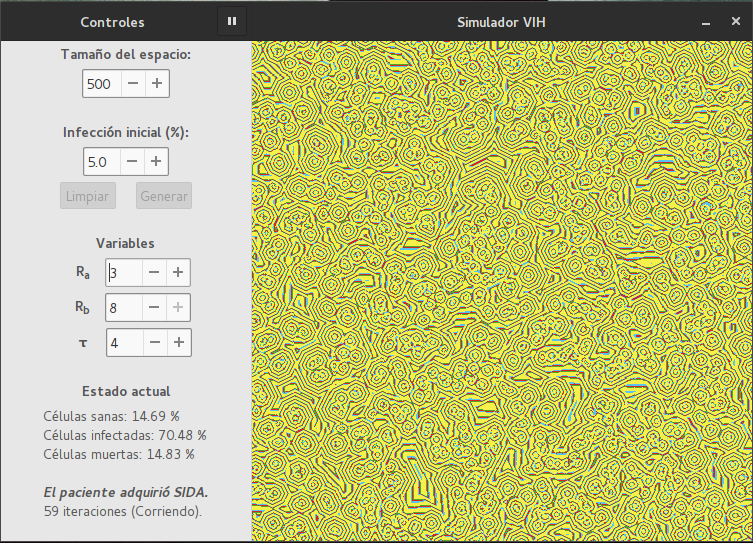
\includegraphics[width=8cm]{img/resistencia/max/2.png} \\
		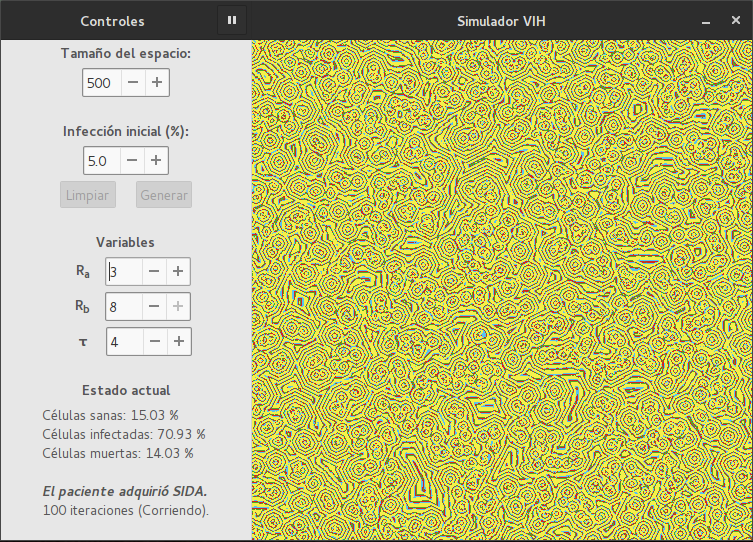
\includegraphics[width=8cm]{img/resistencia/max/3.png} & 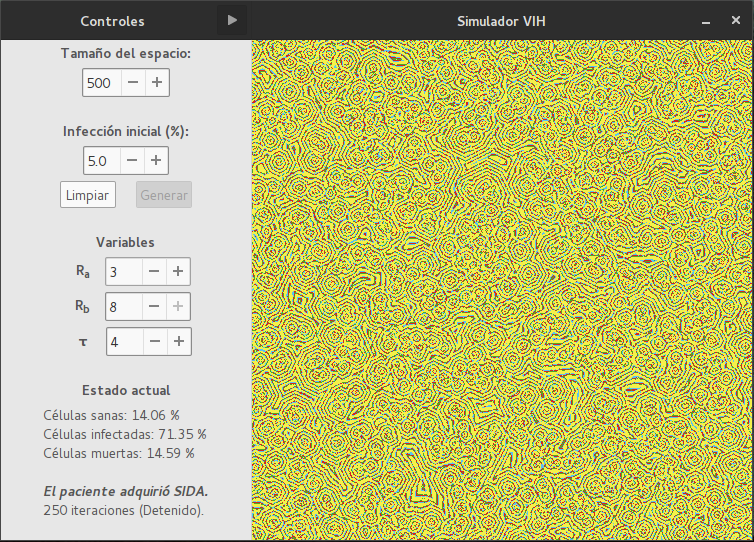
\includegraphics[width=8cm]{img/resistencia/max/4.png} \\
		\end{tabular}
	\end{center}

	\subsubsection{Gráfica de densidades}
	\begin{center}
		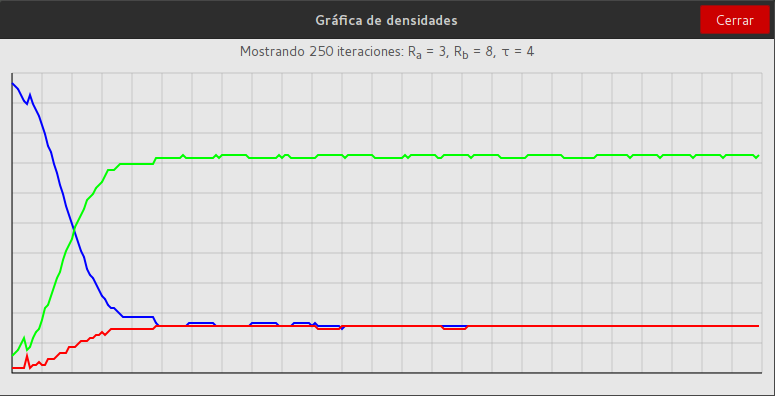
\includegraphics[width=14cm]{img/resistencia/max/g.png}
	\end{center}
	% subsection resistencia_celular_m_xima (end)
	% section casos_extremos (end)
	
	\chapter{Variando el tiempo de respuesta inmunológica}
	\section{Menor tiempo de respuesta inmunológica} % (fold)
	\label{sec:menor_tiempo_de_respuesta_inmunol_gica}
	\begin{center}
		\begin{tabular}{c c}
		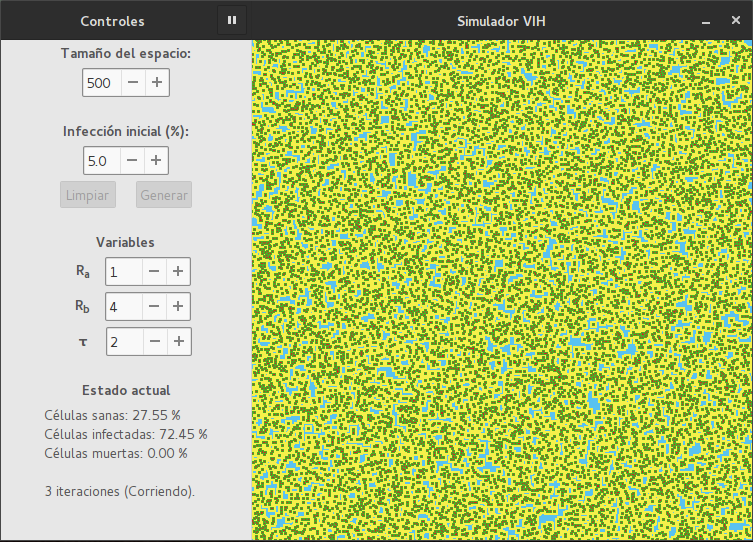
\includegraphics[width=8cm]{img/tiempo/prueba/baja/1.png} & 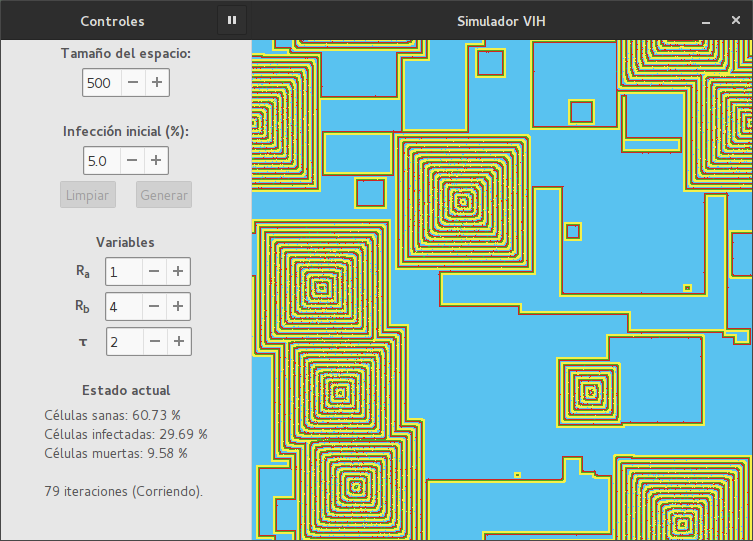
\includegraphics[width=8cm]{img/tiempo/prueba/baja/2.png} \\
		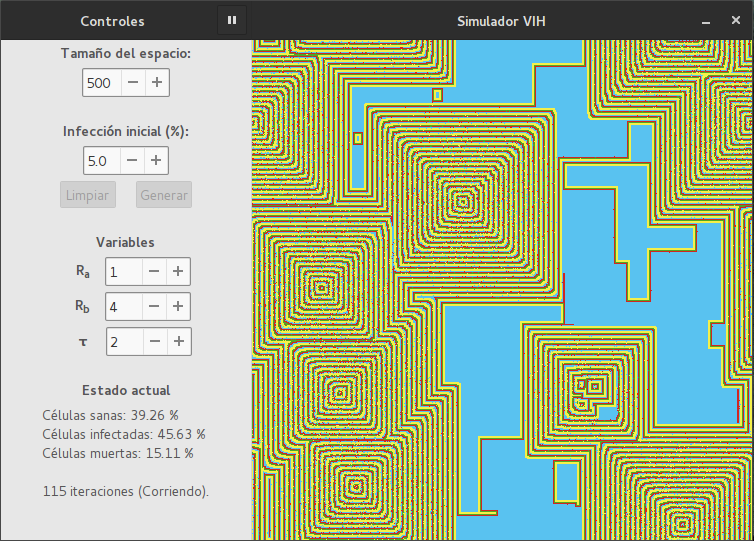
\includegraphics[width=8cm]{img/tiempo/prueba/baja/3.png} & 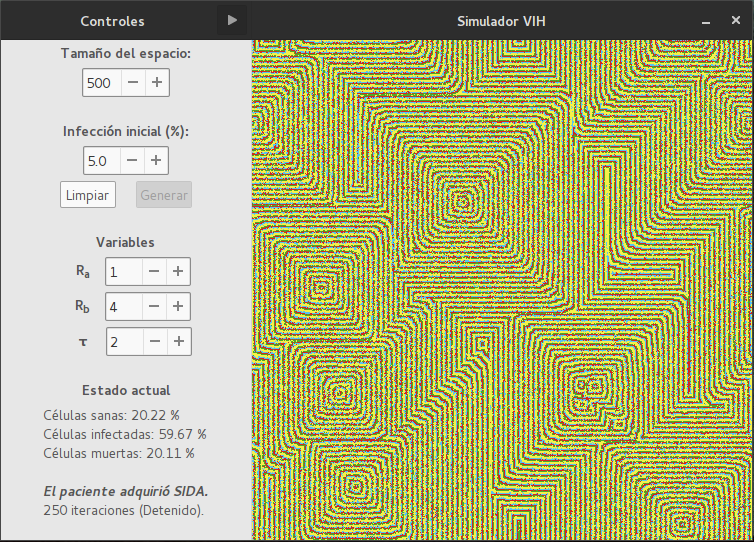
\includegraphics[width=8cm]{img/tiempo/prueba/baja/4.png} \\
		\end{tabular}
	\end{center}

	\subsubsection{Gráfica de densidades}
	\begin{center}
		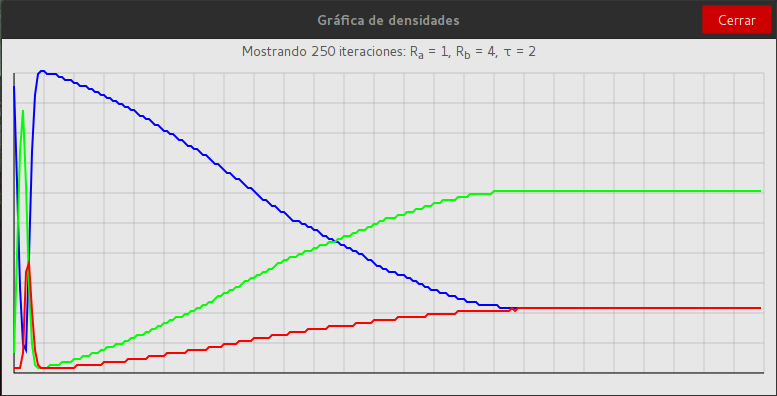
\includegraphics[width=14cm]{img/tiempo/prueba/baja/g.png}\\[3cm]
	\end{center}
	% section menor_tiempo_de_respuesta_inmunol_gica (end)

	\section{Mayor tiempo de respuesta inmunológica} % (fold)
	\label{sec:mayor_tiempo_de_respuesta_inmunol_gica}
	\begin{center}
		\begin{tabular}{c c}
		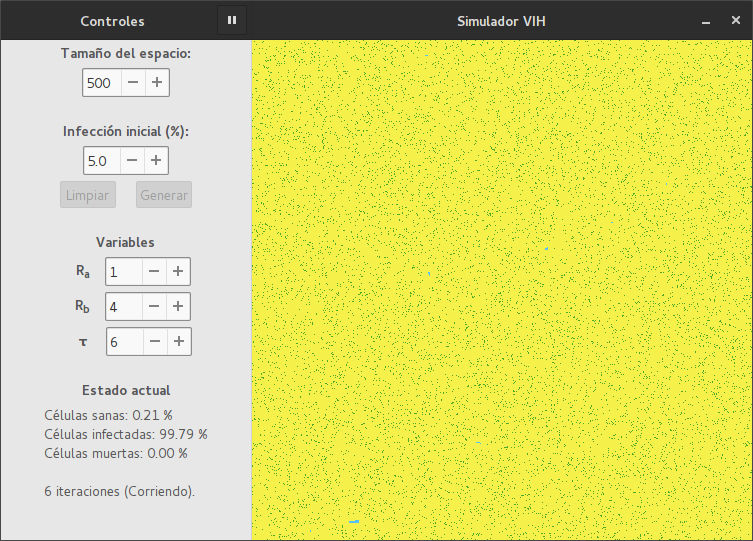
\includegraphics[width=8cm]{img/tiempo/prueba/alta/1.png} & 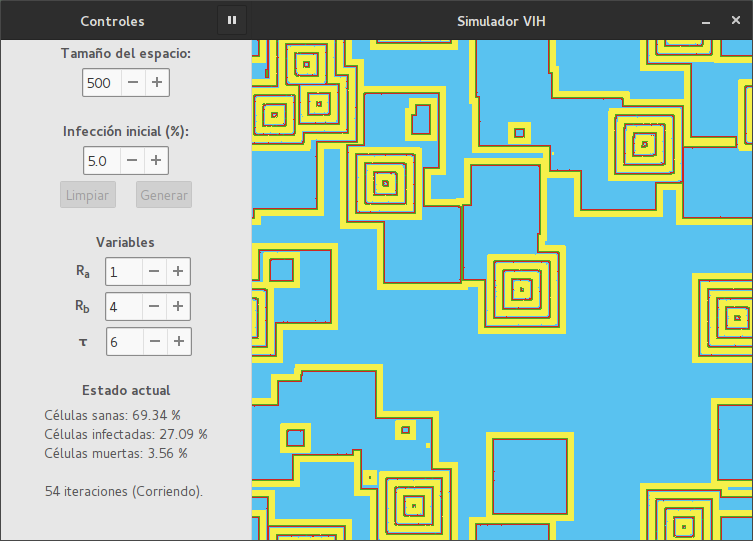
\includegraphics[width=8cm]{img/tiempo/prueba/alta/2.png} \\
		\end{tabular}
	\end{center}

	\begin{center}
		\begin{tabular}{c c}
		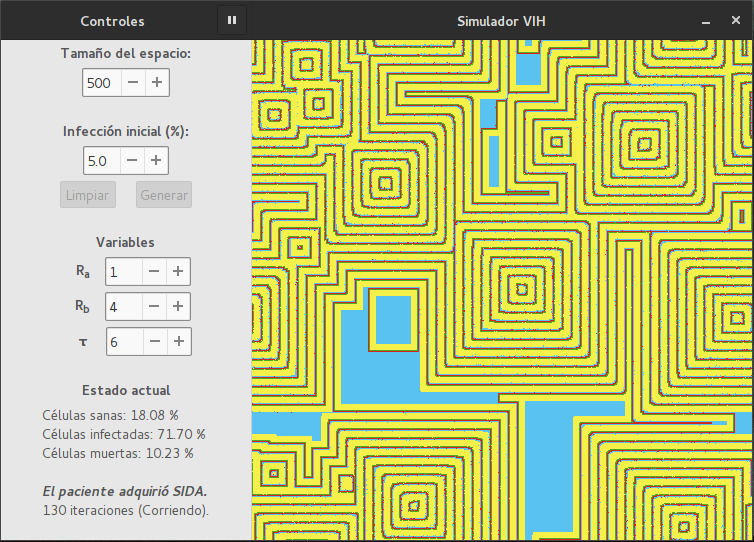
\includegraphics[width=8cm]{img/tiempo/prueba/alta/3.png} & 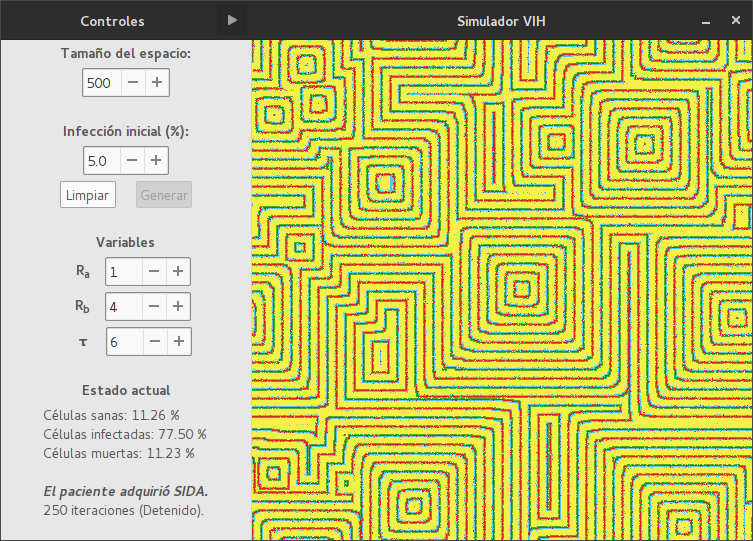
\includegraphics[width=8cm]{img/tiempo/prueba/alta/4.png} \\
		\end{tabular}
	\end{center}

	\subsubsection{Gráfica de densidades}
	\begin{center}
		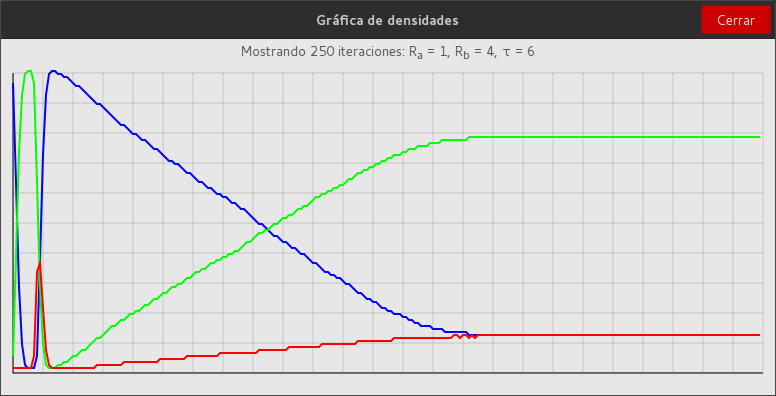
\includegraphics[width=14cm]{img/tiempo/prueba/alta/g.png}
	\end{center}
	% section mayor_tiempo_de_respuesta_inmunol_gica (end)

	\section{Casos extremos} % (fold)
	\label{sec:casos_extremos_3}
	\subsection{Tiempo de respuesta inmunológica mínima} % (fold)
	\label{sub:tiempo_de_respuesta_inmunol_gica_m_nima}
	\begin{center}
		\begin{tabular}{c c}
		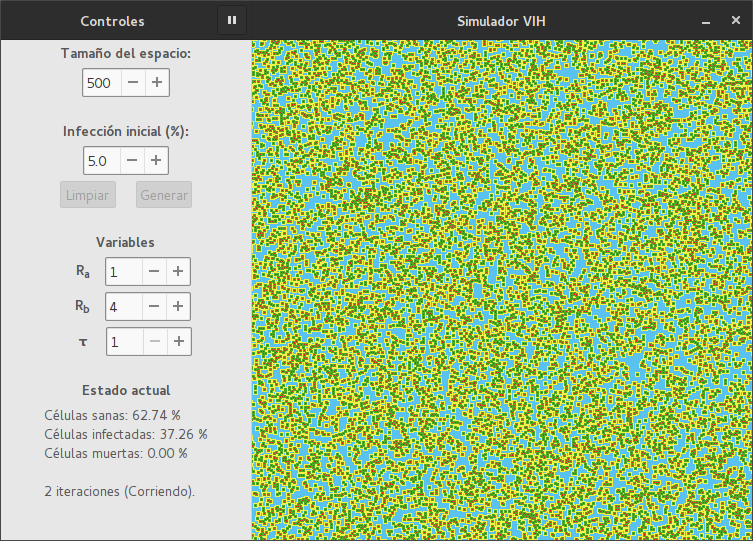
\includegraphics[width=8cm]{img/tiempo/min/1.png} & 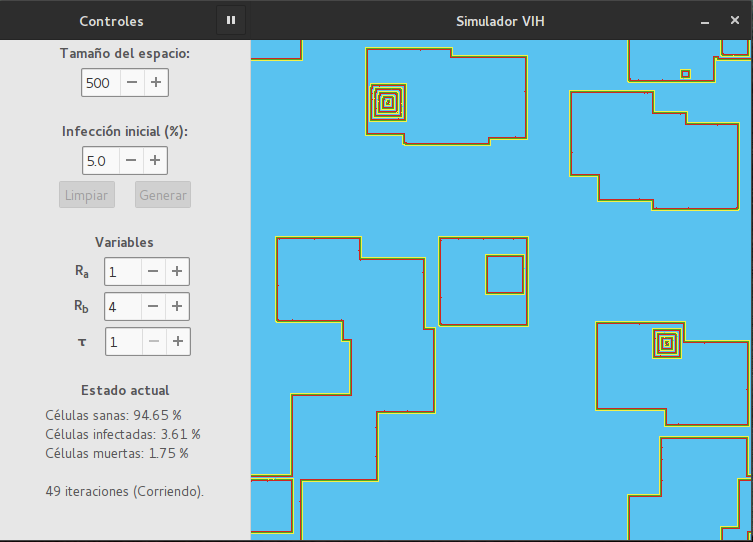
\includegraphics[width=8cm]{img/tiempo/min/2.png} \\
		\includegraphics[width=8cm]{img/tiempo/min/3.png} & \includegraphics[width=8cm]{img/tiempo/min/4.png} \\
		\end{tabular}
	\end{center}

	\subsubsection{Gráfica de densidades}
	\begin{center}
		\includegraphics[width=12cm]{img/tiempo/min/g.png}
	\end{center}
	% subsection tiempo_de_respuesta_inmunol_gica_m_nima (end)

	\subsection{Tiempo de respuesta inmunológica máxima} % (fold)
	\label{sub:tiempo_de_respuesta_inmunol_gica_m_xima}
	\begin{center}
		\begin{tabular}{c c}
		\includegraphics[width=8cm]{img/tiempo/max/1.png} & \includegraphics[width=8cm]{img/tiempo/max/2.png} \\
		\includegraphics[width=8cm]{img/tiempo/max/3.png} & \includegraphics[width=8cm]{img/tiempo/max/4.png} \\
		\end{tabular}
	\end{center}

	\subsubsection{Gráfica de densidades}
	\begin{center}
		\includegraphics[width=14cm]{img/tiempo/max/g.png}
	\end{center}
	% subsection tiempo_de_respuesta_inmunol_gica_m_xima (end)
	% section casos_extremos (end)


	\chapter{Conclusión}
	Podemos observar en el comportamiento por defecto del modelo es el esperado, se forman estructuras de células infectadas rodeando a las células sanas, en la gráfica de densidades podemos observar la fase de infección, donde se nota un incremento de casi el 100\% en las células infectadas y la fase de latencia donde notamos un decremento constante de células sanas.\\

	Al momento de cambiar la infección inicial al mínimo el comportamiento no cambia demasiado, solamente aumenta la duración de la fase de latencia unas cuantas iteraciones y la densidad de las células infectadas no llega a ser tan alta durante la fase de infección. En el caso de la infección inicial al máximo la única diferencia es que la fase de latencia dura unas cuantas iteraciones menos.\\

	Al variar la resistencia celular y hacerla un poco más baja el comportamiento en el autómata no varía demasiado y en la gráfica de densidades podemos ver el resultado esperado, el periodo de latencia del virus se hace significativamente más corto. Sin embargo al aumentar la resistencia celular un poco el comportamiento del autómata cambia y deja de formar las estructuras cuadradas que se habían visto hasta ahora, además que en la gráfica de densidades podemos observar un comportamiento contrario al esperado, la densidad de las células infectadas aumenta de forma bastante acelerada y se mantiene casi constante a partir de alcanzar un cierto porcentaje (en este caso, poco más del 70\%). En los casos extremos podemos ver reflejado estos mismos comportamientos ligeramente exagerados.\\

	Al variar el tiempo de respuesta inmunológica y hacerlo más bajo podemos notar que el comportamiento del autómata es parecido al normal excepto que la propagación del virus se hace más lenta (como era de esperarse) y esto lo podemos observar en la gráfica de densidades. De igual manera, al aumentar el tiempo de respuesta podemos ver que la propagación ocurre más rápidamente. Luego, en los casos extremos, con el tiempo de respuesta mínimo la propagación ocurre de manera aún más lentamente, sin embargo al aumentarlo al máximo podemos ver que la densidad de las células infectadas es mayor pero la propagación ocurre más lentamente que en el caso anterior (con $\tau = 6$).\\

	


    \begingroup
	\renewcommand{\cleardoublepage}{}
	\renewcommand{\clearpage}{}
	\chapter{Referencias}
	\begin{enumerate}
		\item Solovey G., Peruani F., Ponce S., Zorzenon R. ``On cell resistance and inmune response time lag in a model for the HIV infection''. Physica A 343 (2004). Págs. 543 - 556.\\
		\item Zorzenon R., Coutinho S. ``Dynamics of HIV infection: A cellular automata approach''. Physical Review Letters (2001), Vol. 87, No. 16.
	\end{enumerate}
	\endgroup
\end{document}